%%
%  ******************************************************************************
%  * #file    Szablon_raportu_EN_Latex.tex
%  * #author  Adrian Wójcik   adrian.wojcik(at)put.poznan.pl
%  *          
%  * #commit  Patryk Kościk   koscikpatryk(at)gmail.com
%  *          Modified the template for Projekt przejsciowy purposes          
%  *          
%  *
%  * #commit  Patryk Kościk   koscikpatryk(at)gmail.com
%  *          Zupełnie przewrócono na łeb formatke po taktycznym wyjasnieniu          
%  *          
%  * #version 1.1
%  * #date    09-Mar-2022
%  * #brief   PROJPRZEJ
%  *
%  ******************************************************************************
%%  
\documentclass[11pt, a4paper]{article}

\usepackage{SM_template}

% Wypełnijcie te dyrektywy zgodnie z waszym tematem
%
% \lab      -> NAZWA CZUJNIKA,          np.: 'DHT22'
% \comment  -> Króciutki opis co to,    np.: 'Cyfrowy czujnik temperatury'
% \author   -> Autor dokumentu          np.: Patryk Kościk
%
% Pamiętajcie o zmianie ścieżki w \addbibresourcue (!)

\lab{Joystick}
\comment{Moduł sterowania analogowego}
\author{Dawid Sobczak}
\addbibresource{bib/Joystick.bib}
%
% Początek dokumentu
%
\begin{document}

%
% Strona tytułowa
%
\mainpage{Joystick/joystick_module.PNG}
\newpage

\section*{Opis elementu}
Głównym elementem składającym się na moduł joystick-a są dwa potencjometry obrotowe B103 267 ustawione względem siebie pod kątem 90 stopni. Potencjometr ten charakteryzuje się rezystancją w zakresie od około 0 do 10k [$\Omega$]. Rezystancja zależna jest od położenia kątowego potencjometru. Dodatkowy element w module - przycik (ang. push-button) w układzie NO (ang. Normaly-Open).
%%%%%%%%%%%%%%%%%%%%%%%%%  TWO IMAGES SIDE BY SIDE  %%%%%%%%%%%%%%%%%%%%%%%%%%%%%
\vspace{0.25cm}
\begin{figure}[h]
\centering
%%%%%%%%%%%%%%%%%%%%%%%%%%%%%%%%%%%%%%%%%%%%%%%%%%%%%%%%%%%%%%%%%%%%%%%%%%%%%%%%%
\begin{subfigure}{.5\textwidth}
\centering
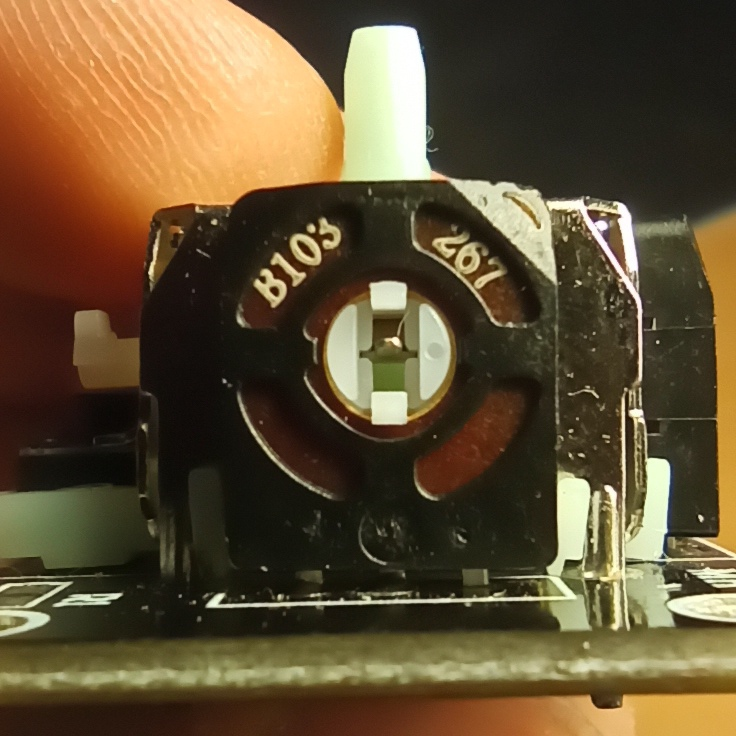
\includegraphics[width=.6\linewidth]{fig/Joystick/b103.jpg}
\caption{\centering Wykorzystany potencjometr obrotowy \\
10k - B103 267}
\label{fig:_zdjecie_elementu}
\end{subfigure}%
%%%%%%%%%%%%%%%%%%%%%%%%%%%%%%%%%%%%%%%%%%%%%%%%%%%%%%%%%%%%%%%%%%%%%%%%%%%%%%%%%
\begin{subfigure}{.5\textwidth}
\centering
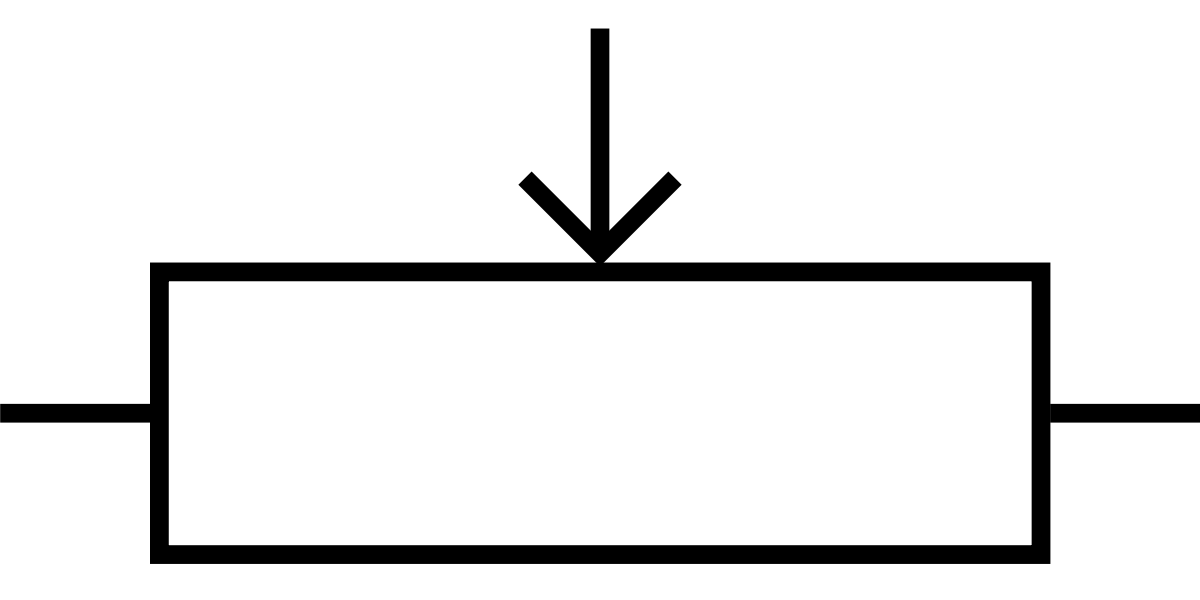
\includegraphics[width=.6\linewidth]{fig/Joystick/potentiometer_schematic.png}
\caption{Zapis symboliczny potencjometru}
\label{fig:_zasada_dzialania_elementu}
\end{subfigure}
%%%%%%%%%%%%%%%%%%%%%%%%%%%%%%%%%%%%%%%%%%%%%%%%%%%%%%%%%%%%%%%%%%%%%%%%%%%%%%%%%
\label{fig:element}
\end{figure}
\vspace{0.25cm}

Moduł zasilany napięciem 3.3 - 5.0 V ma wyprowadzenia w postaci trzech sygnałów, odpowiadających kolejno za pozycję X, pozycję Y oraz stan logiczny obwodu przycisku. Manipulowanie centralnie umieszczonym drążkiem w dwóch osiach powoduje zmianę pozycji kątowej potencjometrów oraz zmienę ich rezystancję. W konsekwencji tego działania i faktu użycia potencjometrów w układach dzielników napięcia, zmienia się napięcie odpowiednio na wyjściach analogowych VRX oraz VRY. Przyciśnięcie drążka do podstawy modułu powoduje zwarcie obwodu przycisku oraz wystawienie na pinie SW stanu wysokiego.
%%%%%%%%%%%%%%%%%%%%%%%%%  TWO IMAGES SIDE BY SIDE  %%%%%%%%%%%%%%%%%%%%%%%%%%%%%
% \subsection{Opis modułu} REPLACE SUBSECTION WITH 1CM VSPACE
\vspace{0.75cm}
%%%%%%%%%%%%%%%%%%%%%%%%%  TWO IMAGES SIDE BY SIDE  %%%%%%%%%%%%%%%%%%%%%%%%%%%%%
\begin{figure}[h]
\centering
%%%%%%%%%%%%%%%%%%%%%%%%%%%%%%%%%%%%%%%%%%%%%%%%%%%%%%%%%%%%%%%%%%%%%%%%%%%%%%%%%
\begin{subfigure}{.5\textwidth}
\centering
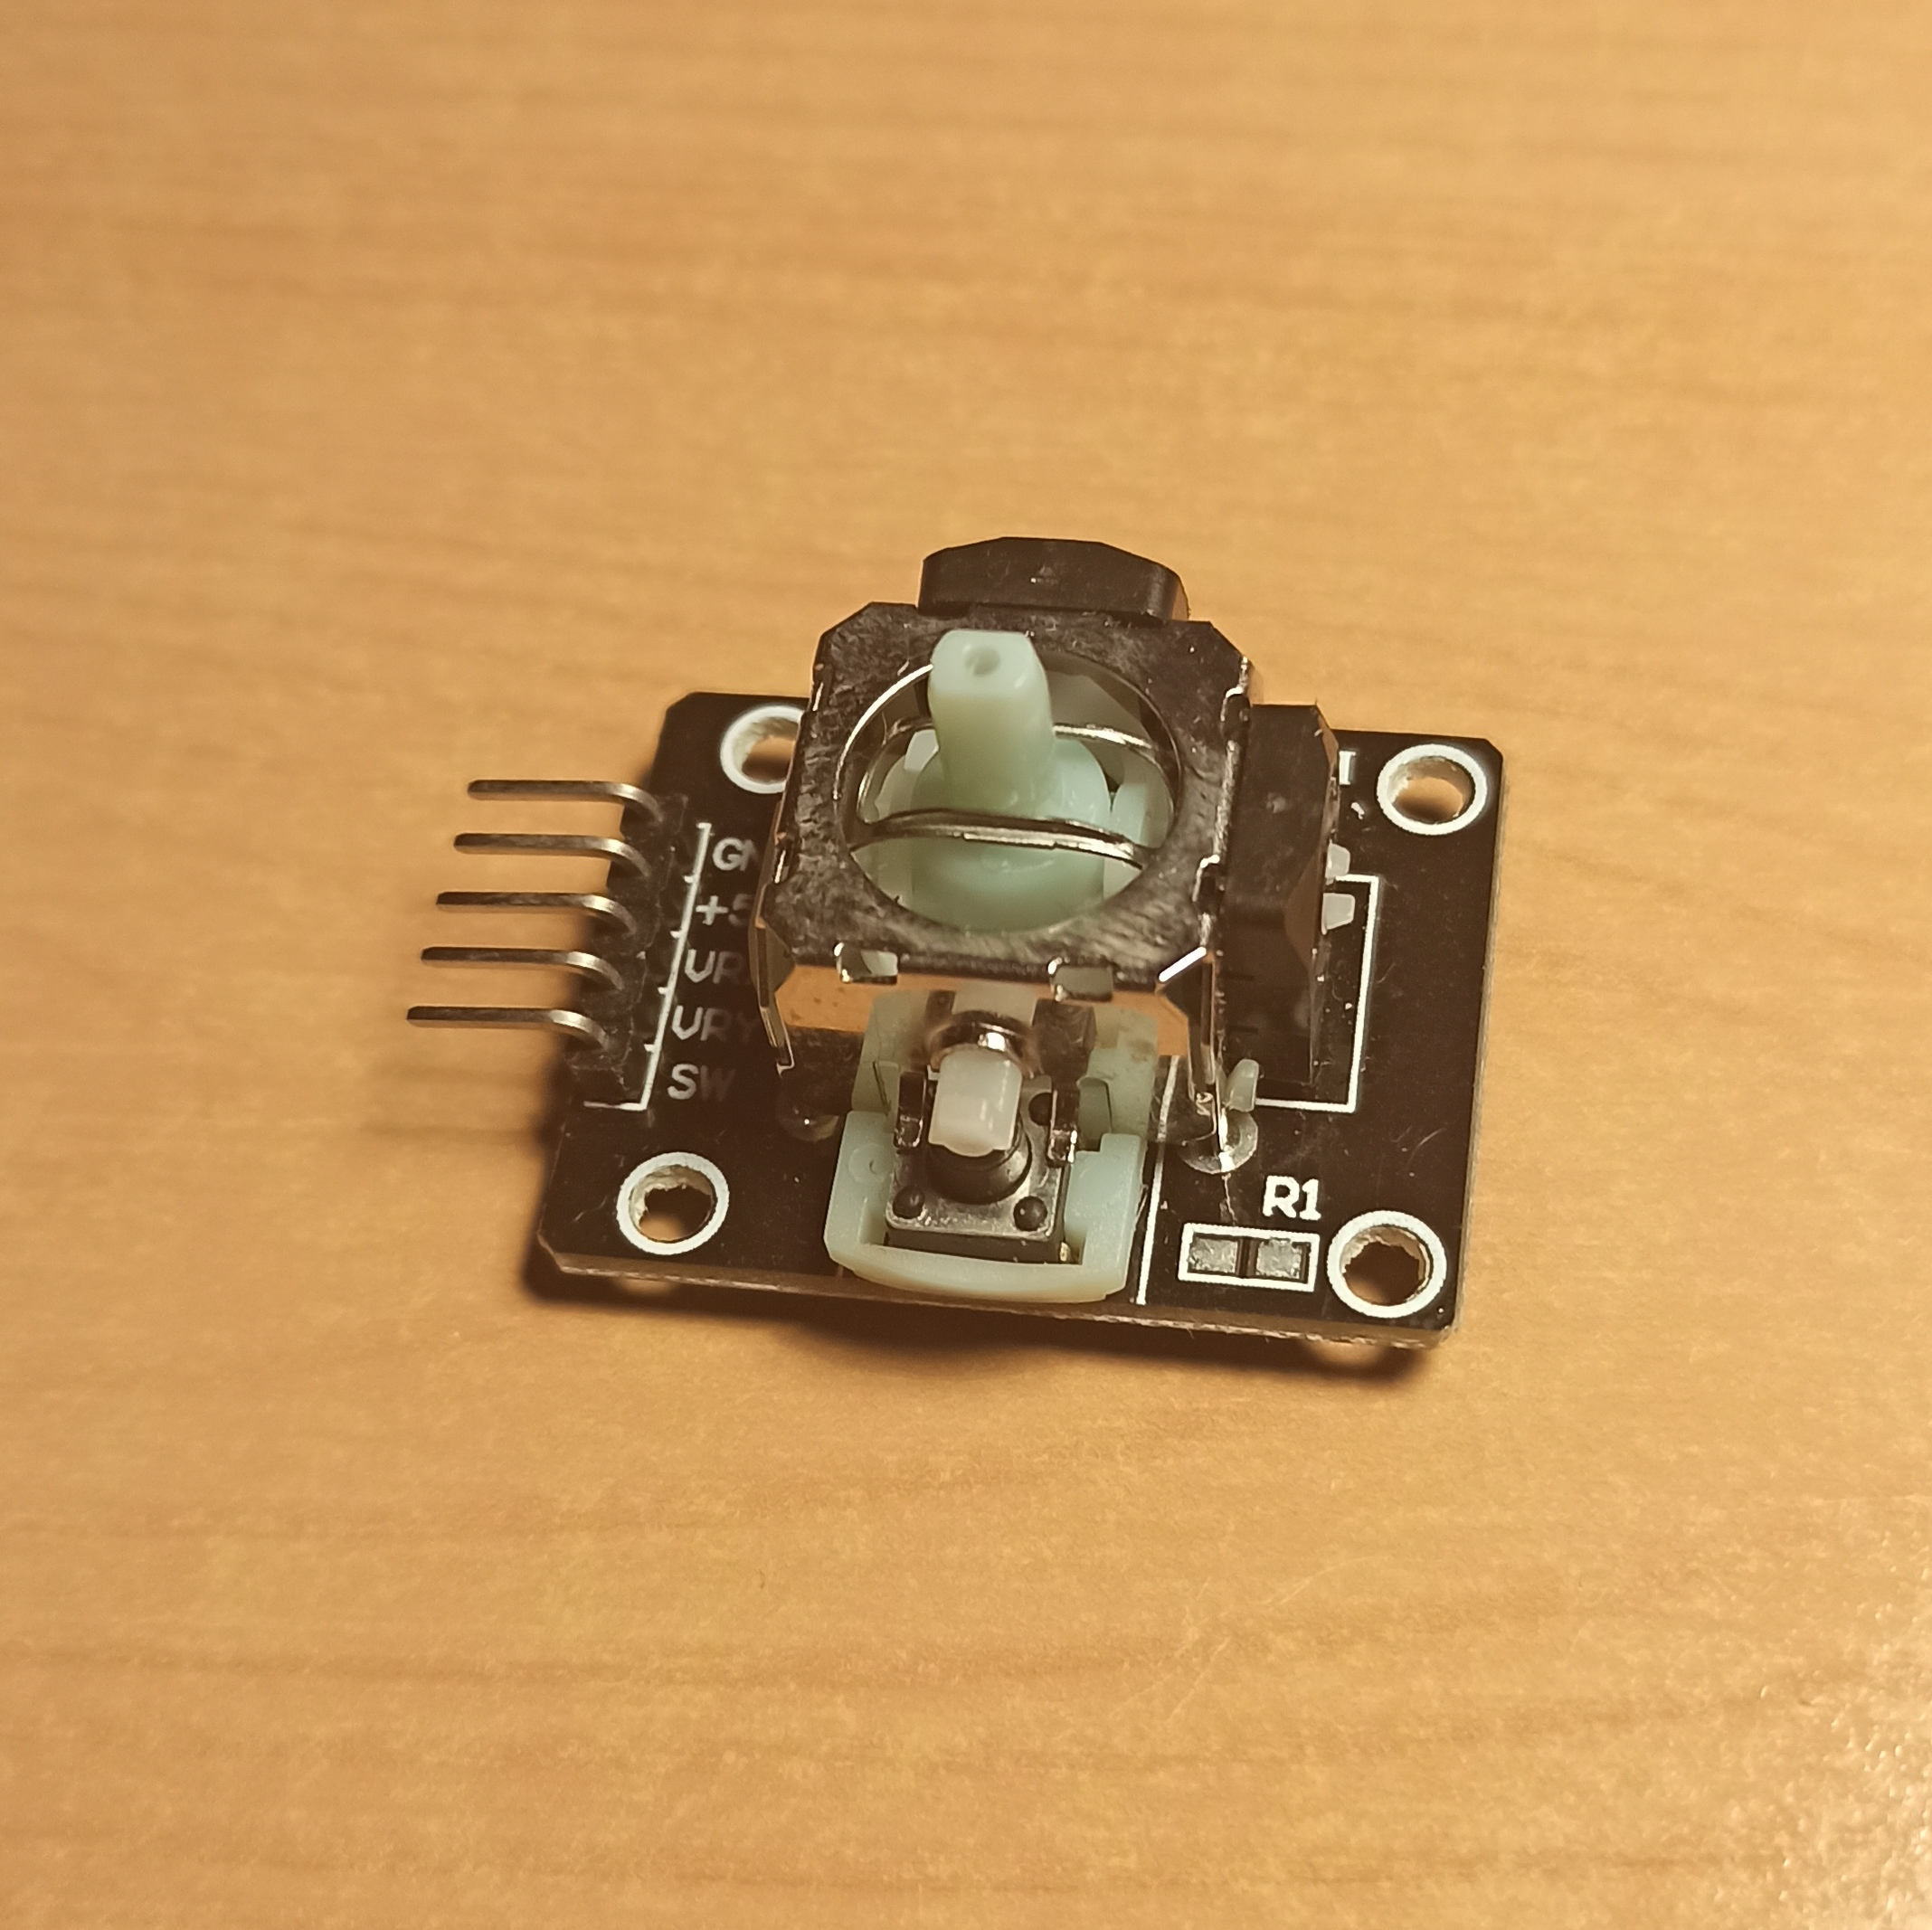
\includegraphics[width=.6\linewidth]{fig/Joystick/joystick_photo.jpg}
\caption{Zdjęcie modułu Joystick}
\label{fig:_zdjecie_modulu}
\end{subfigure}%
%%%%%%%%%%%%%%%%%%%%%%%%%%%%%%%%%%%%%%%%%%%%%%%%%%%%%%%%%%%%%%%%%%%%%%%%%%%%%%%%%
\begin{subfigure}{.5\textwidth}
\centering
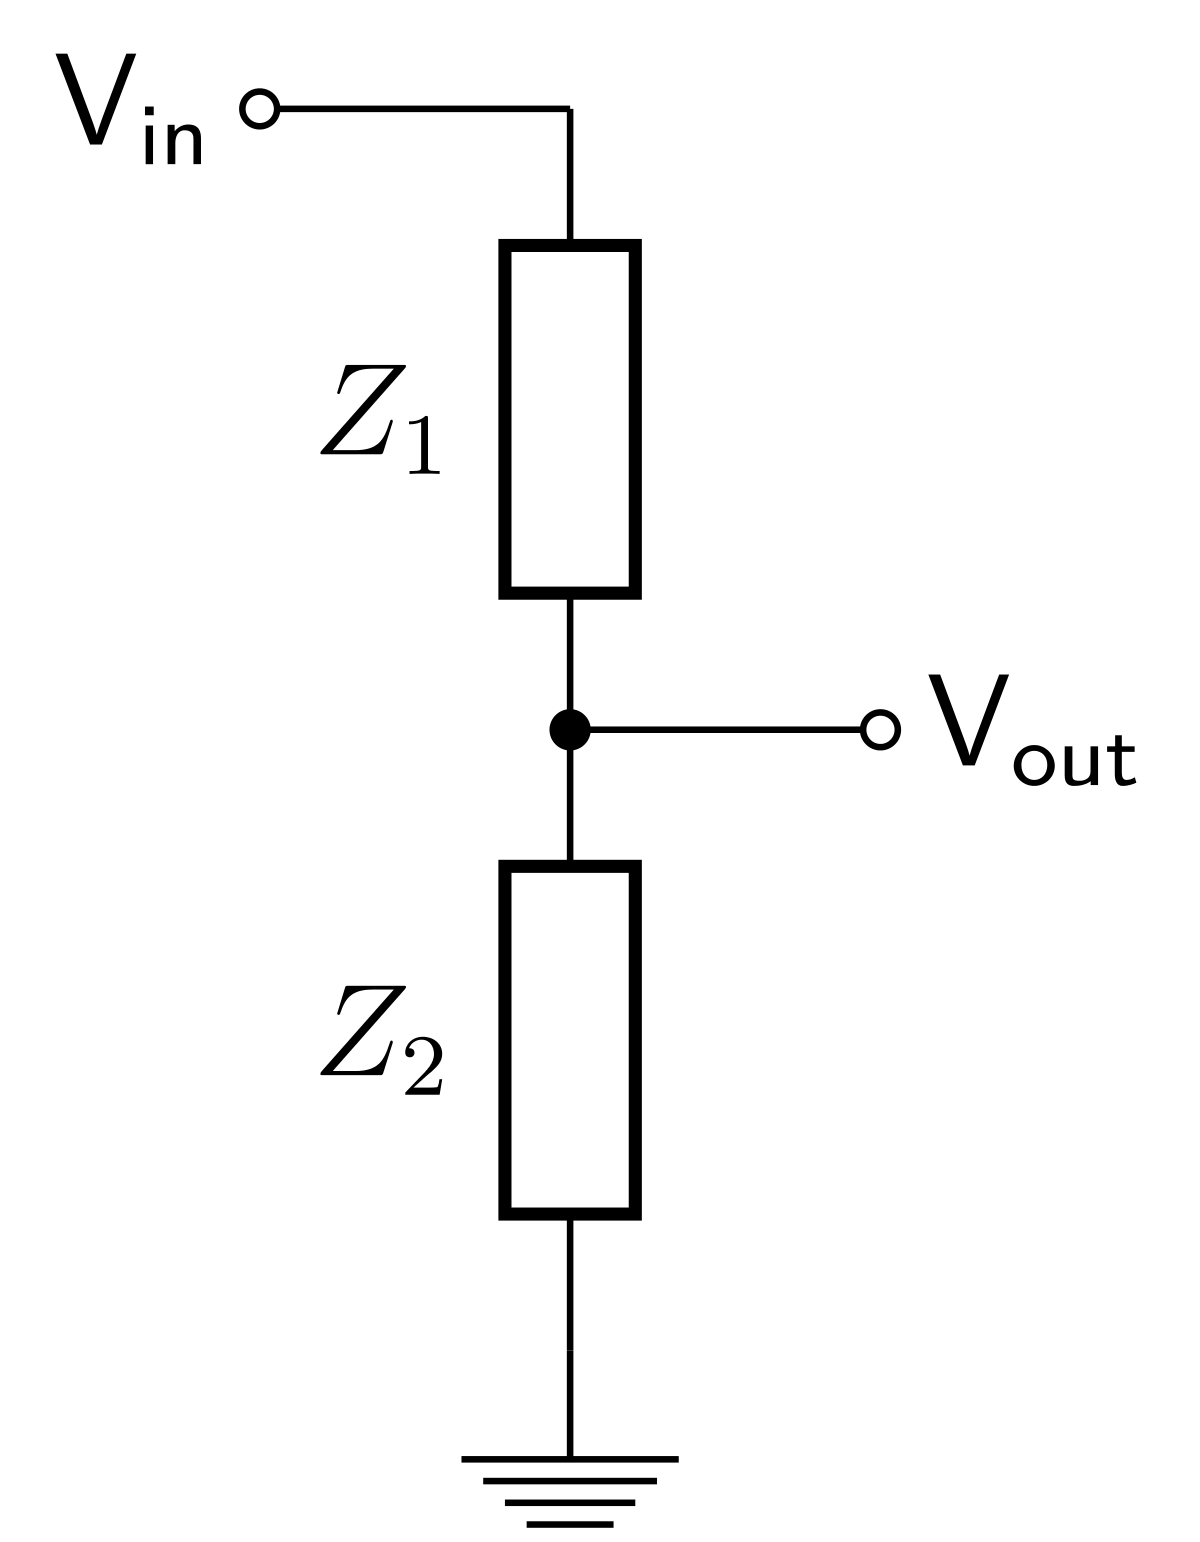
\includegraphics[width=.5\linewidth]{fig/Joystick/voltage_divider_schematic.png}
\caption{Schemat dzielnika napięcia}
\label{fig:_schemat_modulu}
\end{subfigure}
%%%%%%%%%%%%%%%%%%%%%%%%%%%%%%%%%%%%%%%%%%%%%%%%%%%%%%%%%%%%%%%%%%%%%%%%%%%%%%%%%
\label{fig:modul}
\end{figure}
\vspace{0.5cm}
%%%%%%%%%%%%%%%%%%%%%%%%%  TWO IMAGES SIDE BY SIDE  %%%%%%%%%%%%%%%%%%%%%%%%%%%%%

Warto zaznaczyć, że zakres napięcia zwracanego na pinach VRX oraz VRY zamyka się w przedziałach $<0, +3.3>$ (lub $<0, +5.0>$)[V] . Drążek, ze względu na zastosowanie mechanicznych sprężyn, pozycję bazową ma na środku obszaru ruchu, określanego odpowiednio przez napięcie 1.65 [V], czyli połowę napięcia zasilającego moduł.



\newpage
\begin{figure}[h]
    \centering
    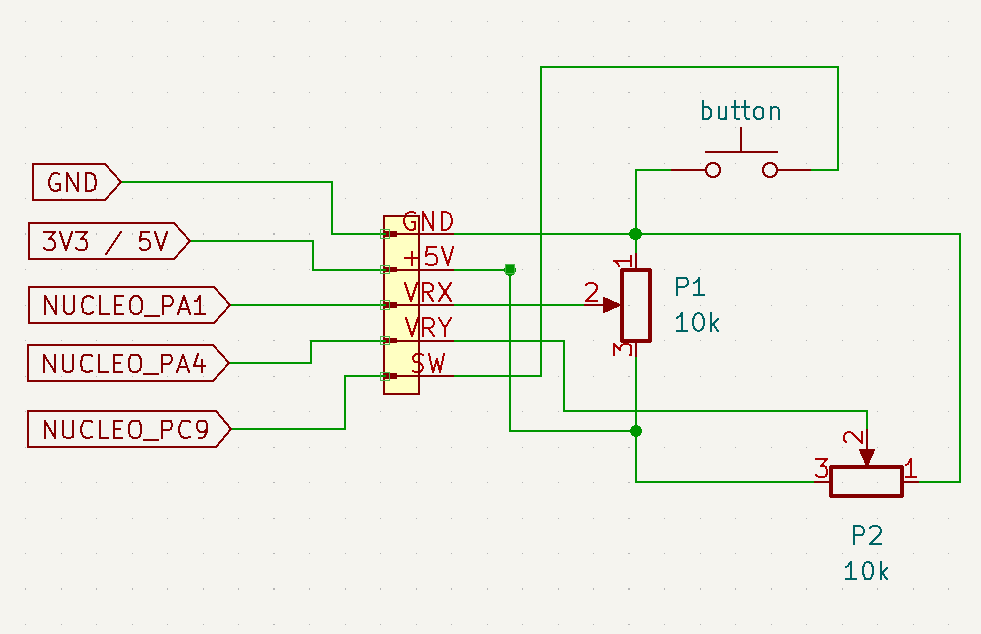
\includegraphics[width=0.8\textwidth]{fig/Joystick/joystick_schematic.PNG}
    \caption{Ogólny schemat elektryczny modułu Joystick-a}
\end{figure}
\newpage
\section{Użycie modułu}
\subsection{Bez mikrokontrolera}
Działanie modułu można w najprostszy sposób sprawdzić przy wykorzystaniu multimetru w trybie woltomierza, do pinów VRX lub VRY. Dodatkowo można sprawdzić poprawność działania przycisku, podłączając do wyprowadzenia SW multimetr w trybie badania ciągłości obwodu (z brzęczykiem).
\vspace{0.5cm}
% TUTAJ FOTY ODNOSNIE TEGO
%%%%%%%%%%%%%%%%%%%%%%%%%  TWO IMAGES SIDE BY SIDE  %%%%%%%%%%%%%%%%%%%%%%%%%%%%%
\vspace{0.25cm}
\begin{figure}[h]
\centering
%%%%%%%%%%%%%%%%%%%%%%%%%%%%%%%%%%%%%%%%%%%%%%%%%%%%%%%%%%%%%%%%%%%%%%%%%%%%%%%%%
\begin{subfigure}{.5\textwidth}
\centering
\includegraphics[width=.9\linewidth]{fig/Joystick/home.jpg}
\caption{\centering Wskazanie multimetru dla pozycji 'home' joysticka}
\label{fig:_uklad_woltomierz_otw}
\end{subfigure}%
%%%%%%%%%%%%%%%%%%%%%%%%%%%%%%%%%%%%%%%%%%%%%%%%%%%%%%%%%%%%%%%%%%%%%%%%%%%%%%%%%
\begin{subfigure}{.5\textwidth}
\centering
\includegraphics[width=.9\linewidth]{fig/Joystick/max_y.jpg}
\caption{\centering Wskazanie multimetru przy maksymalnym odchyleniu drążka w osi Y}
\label{fig:_uklad_woltomierz_zmk}
\end{subfigure}
%%%%%%%%%%%%%%%%%%%%%%%%%%%%%%%%%%%%%%%%%%%%%%%%%%%%%%%%%%%%%%%%%%%%%%%%%%%%%%%%%
% \caption{PODPIS}
\label{fig:woltomierz}
\end{figure}
\vspace{0.25cm}
%%%%%%%%%%%%%%%%%%%%%%%%%  TWO IMAGES SIDE BY SIDE  %%%%%%%%%%%%%%%%%%%%%%%%%%%%%
\vspace{0.5cm}

%%%%%%%%%%%%%%%%%%%%%%%%%  TWO IMAGES SIDE BY SIDE  %%%%%%%%%%%%%%%%%%%%%%%%%%%%%
\vspace{0.25cm}
\begin{figure}[h]
\centering
%%%%%%%%%%%%%%%%%%%%%%%%%%%%%%%%%%%%%%%%%%%%%%%%%%%%%%%%%%%%%%%%%%%%%%%%%%%%%%%%%
\begin{subfigure}{.5\textwidth}
\centering
\includegraphics[width=.9\linewidth]{fig/Joystick/min_y.jpg}
\caption{\centering Wskazanie multimetru przy maksymalnym odchyleniu drążka w osi Y - kierunek przeciwny}
\label{fig:_uklad_woltomierz_otw}
\end{subfigure}%
%%%%%%%%%%%%%%%%%%%%%%%%%%%%%%%%%%%%%%%%%%%%%%%%%%%%%%%%%%%%%%%%%%%%%%%%%%%%%%%%%
\begin{subfigure}{.5\textwidth}
\centering
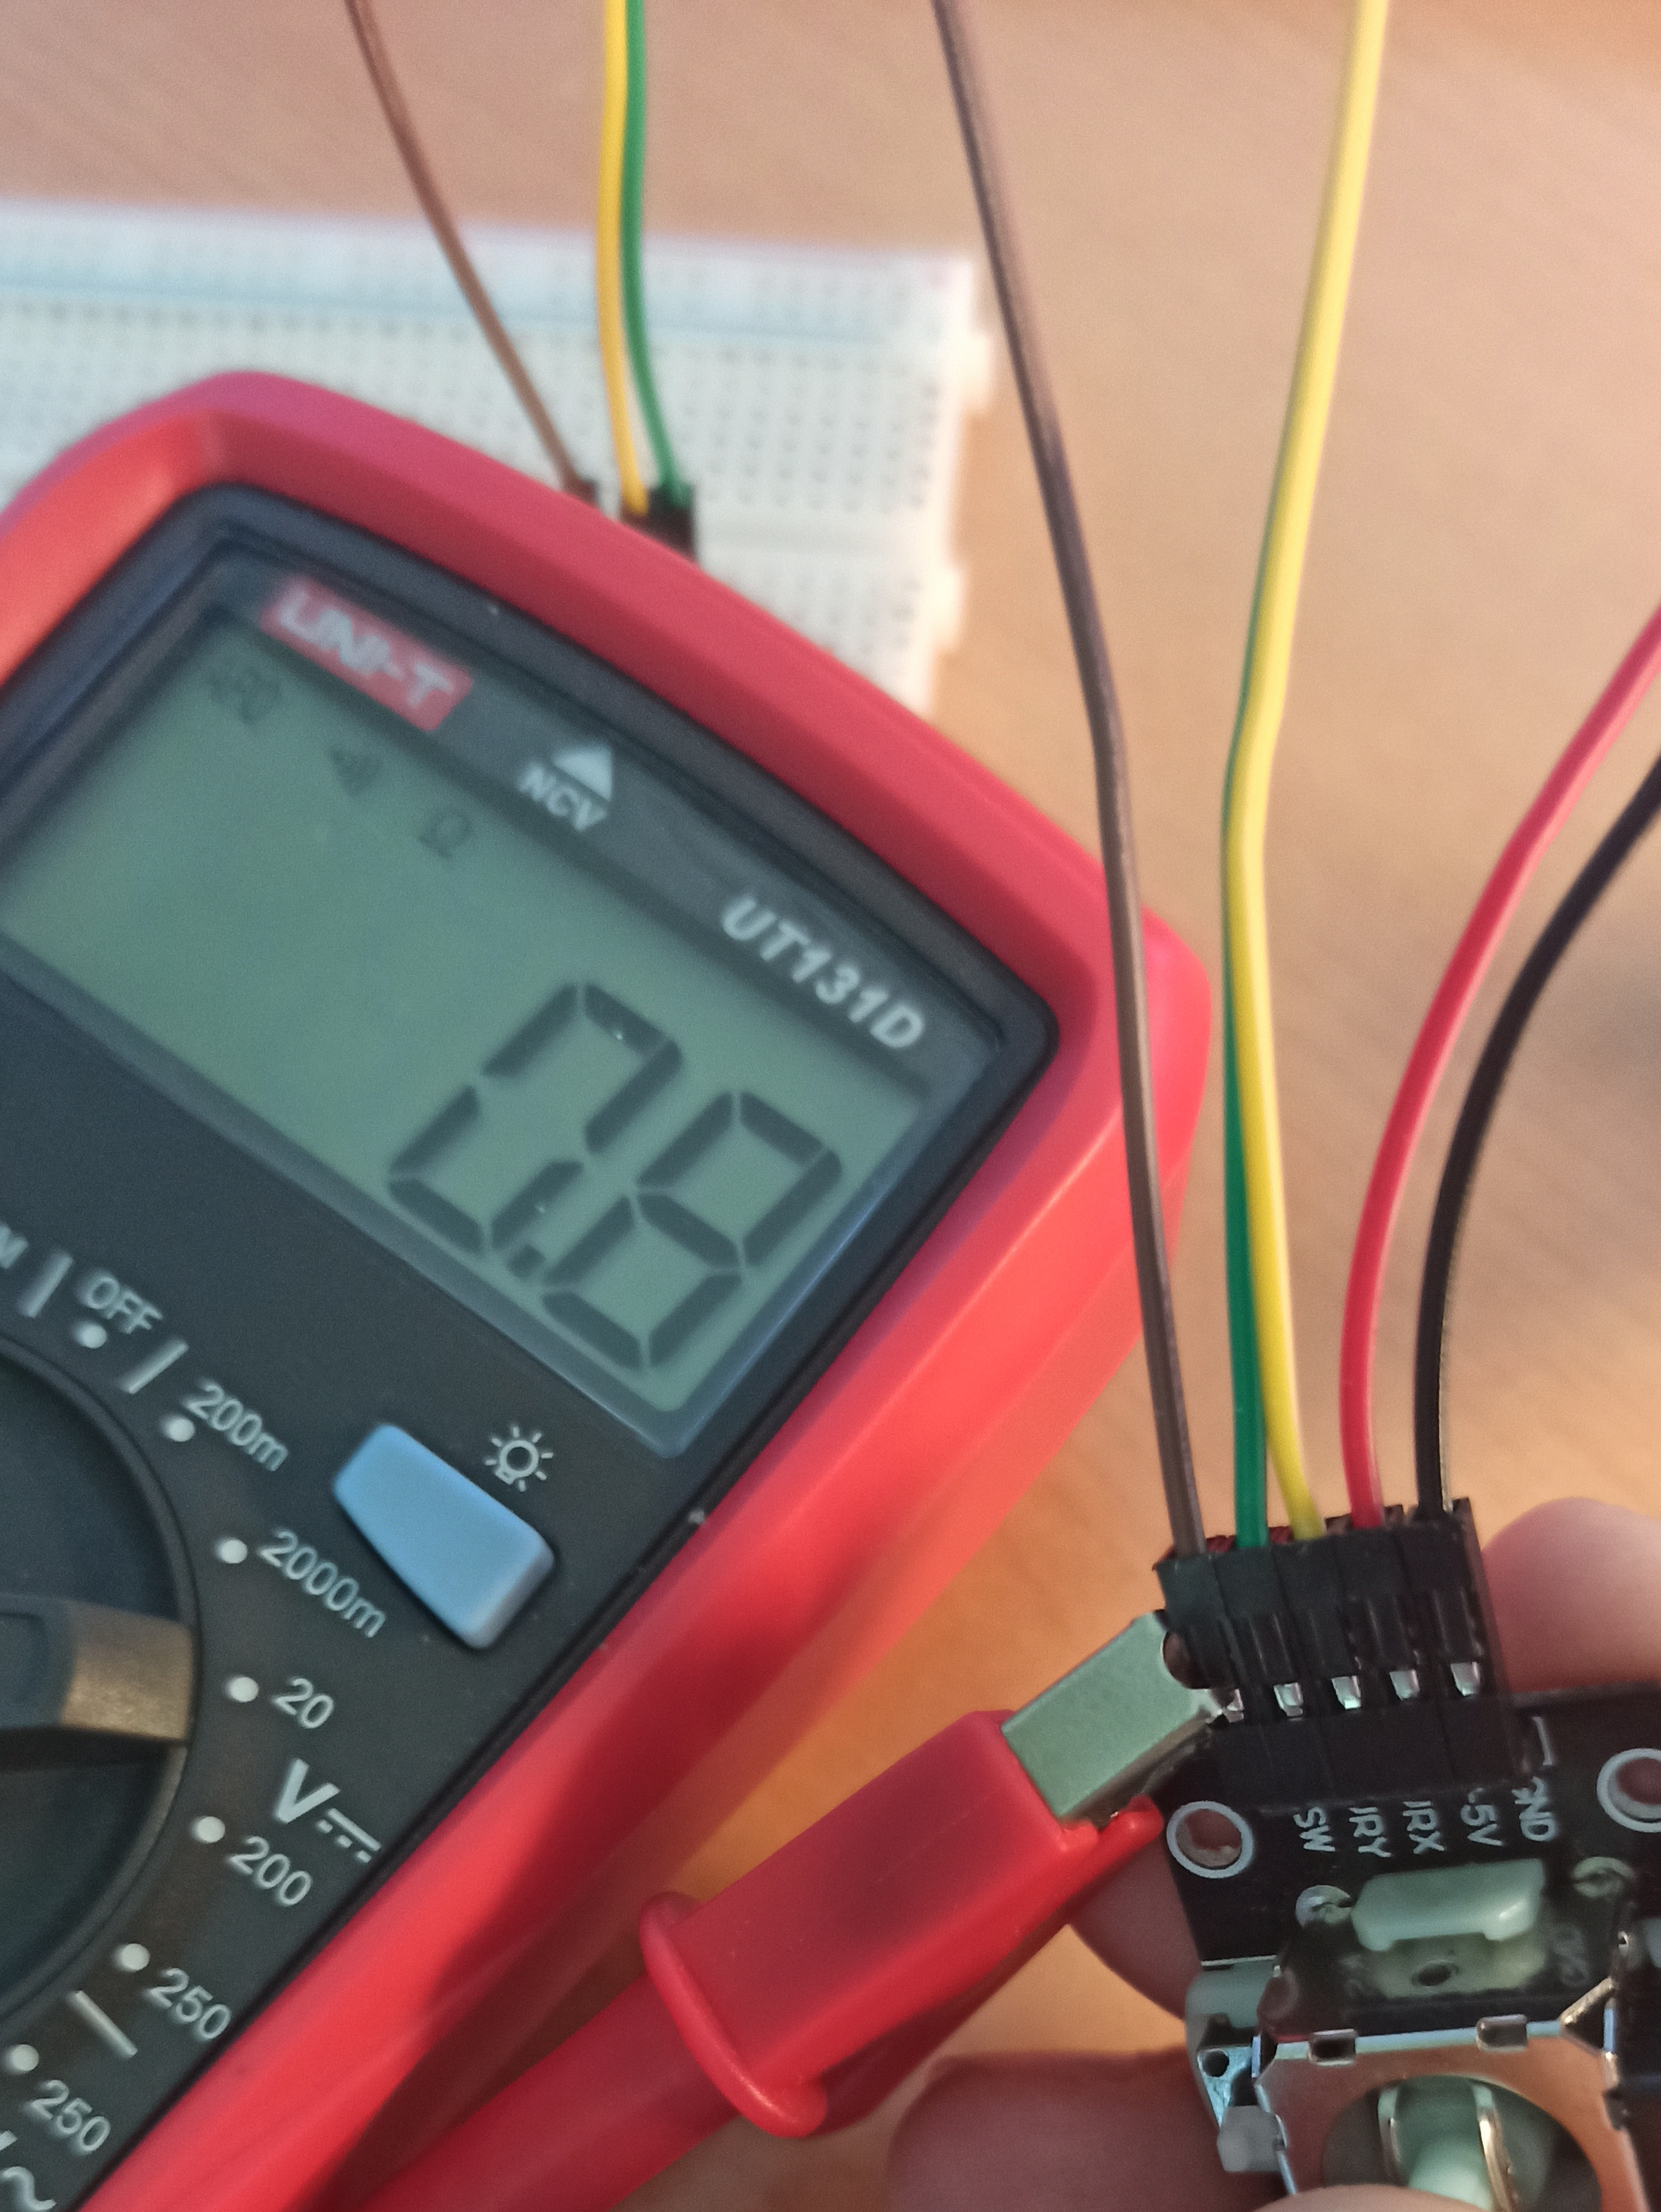
\includegraphics[width=.6\linewidth]{sw.jpg}
\caption{\centering Wskazanie multimetru dla wciśniętego przycisku - obwód zwarty}
\label{fig:_uklad_woltomierz_zmk}
\end{subfigure}
%%%%%%%%%%%%%%%%%%%%%%%%%%%%%%%%%%%%%%%%%%%%%%%%%%%%%%%%%%%%%%%%%%%%%%%%%%%%%%%%%
% \caption{PODPIS}
\label{fig:woltomierz}
\end{figure}
\vspace{0.25cm}
%%%%%%%%%%%%%%%%%%%%%%%%%  TWO IMAGES SIDE BY SIDE  %%%%%%%%%%%%%%%%%%%%%%%%%%%%%
\vspace{0.5cm}
\newpage
\subsection{Mikrokontroler}
Aplikacja modułu wymaga połączenia mikrokontrolera w sposób opisany w tabeli (\ref{tab:tab1}) znajdującej się poniżej. W celu określenia pozycji drążka moduły, wykorzystano dwa kanały przetwornika ADC1 mikrokontrolera.

\vspace{0.5cm}
\begin{table}[h!]
    \centering
    \begin{tabular}{|c|c|c|c|} 
        \hline
        \multicolumn{2}{|c|}{NUCELO-F746ZG} & \multicolumn{2}{c|}{Joystick}  \\ 
        \hline
        Etykieta & Port i numer pinu       & Nr pinu & Etykieta           \\ 
        \hline
        GND      & -                    & 1       & GND             
        \\
        \hline
        3.3V      & -                    & 2        & +5V          
        \\
        \hline
        PA0      & D32                      & 3       & VRX              \\
        \hline
        PA4      & D24                       & 4       & VRY              \\
        \hline
        PC9      & D43                       & 5       & SW              \\
        \hline
    \end{tabular}
    \caption{Połącznie pomiędzy modułem i mikrokontrolerem}
    \label{tab:tab1}
\end{table}

Dodatkowe schematy połączeń i konfiguracja
mikrokontrolera została opisana w sekcji \texttt{Suplement \#1}. Zawiera tam się również kod języka
C + HAL, pozwalający na obsługę modułu.

\vspace{0.5cm}
Działanie układu przedstawiono na załączonym w \texttt{\cite{yt1}} materiale wideo.

\newpage
\printbibliography[heading=bibintoc]

\end{document}